\chapter{Variaciones del Modelo}\label{chap:variaciones}

Teniendo ya claros los conceptos médicos y el análisis de un modelo base acorde con tales conceptos, es momento de introducir al modelo las dos enfermedades presentadas en \ref{sec:RBC:enfermedades}. El caso de las hemorragias es más sencillo que el de la anemia, pues los sangrados son tratados una única vez (hasta que sean frenados), mientras que la anemia es una enfermedad cuyo tratamiento es para toda la vida. En este capítulo se presentarán las variaciones matemáticas del modelo y el análisis de las simulaciones de estas, esperando que los resultados obtenidos logren mantener la homeostasis del paciente y, para el caso de la anemia, ver si un aumento o disminución de la dosis afecta realmente los resultados.

\section{Caso con Hemorragia}\label{Sec:variaciones:hemorragia}

Para los sangrados, se tendrán en cuenta diferentes casos. Inicialmente se tendrá en cuenta una hemorragia leve (pérdida del 2$\%$ de sangre) y se observará lo que sucede si, después de la pérdida de sangre, las variables del modelo se mantienen iguales y que sucede si estas se modifican. Posteriormente se considerará el caso de una hemorragia grave (el 13$\%$ de la sangre del cuerpo) y se observarán los efectos de una transfusión sanguínea para recuperar la homeostasis. En el caso de las hemorragias, se tendrá en cuenta el caso en el que $\gamma =1$, pues así el paciente es totalmente sano, el parámetro $f$ se mantiene igual que antes ($=0.00832$) y los valores iniciales también se mantienen.

\subsection{Hemorragia Leve}\label{subsec:variaciones:hemorragia:leve}

Para esta variación del modelo, considere que en el tercer día de medición el paciente, ya sea por un corte o un accidente, pierde el $2\%$ de su cantidad de sangre en el cuerpo que, considerando el caso de que tenga 5 litros de sangre, esto equivale a 100 mililitros de fluido o a $5\times 10^{11}$ glóbulos rojos. Así, el modelo se puede ver de la siguiente manera:

$$R(n+1)= \left\{ \begin{array}{lcc} (1-f)\cdot R(n)+M(n) & si & n \neq 3 \\ \\ (1-f)\cdot R(n)+M(n)-0.02\cdot R(n) & si & n = 3\end{array} \right.$$
$$M(n+1)=\gamma \cdot f \cdot R(n)$$

En donde:
\begin{itemize}
    \item $\gamma=1$;
    \item $f=0.00832$;
    \item $R(0) = 25\times 10^{12};$
    \item $M(0) = 208 \times 10^{9}.$
\end{itemize}

Así, la simulación se ve así: en la figura \ref{sec:variaciones:fig:HemoLeveG1RBC} se observa la pérdida de RBC's en el tercer día, un aumento del tercero al cuarto y estabilidad del cuarto en adelante. En la figura \ref{sec:variaciones:fig:HemoLeveG1SC} se observa lo mismo pero con un día de atraso. El aumento que se puede observar está dado por el hecho de que el adendo $M(n)$ conserva lo que ha ocurrido en $R(n-1)$ así, para el cuarto día se producen la cantidad de eritrocitos que se vienen produciendo regularmente antes del accidente, y desde el cuarto día en adalente este adendo ya se acomoda a la nueva cantidad de sangre. La estabilidad que se observa del cuarto día en adelante está dada por el hecho de que $\gamma = 1$, el modelo, de esta manera, funciona como lo hace normalmente (véase \ref{subsec:modelo:simulaciones:G1}) tomando una cantidad inicial de sangre menor que la original, es decir que mantiene una estabilidad con la cantidad de RBC's del cuarto día, que es de $24.504\times 10^{12}$ glóbulos rojos. 

\begin{figure}[H]
    \centering
    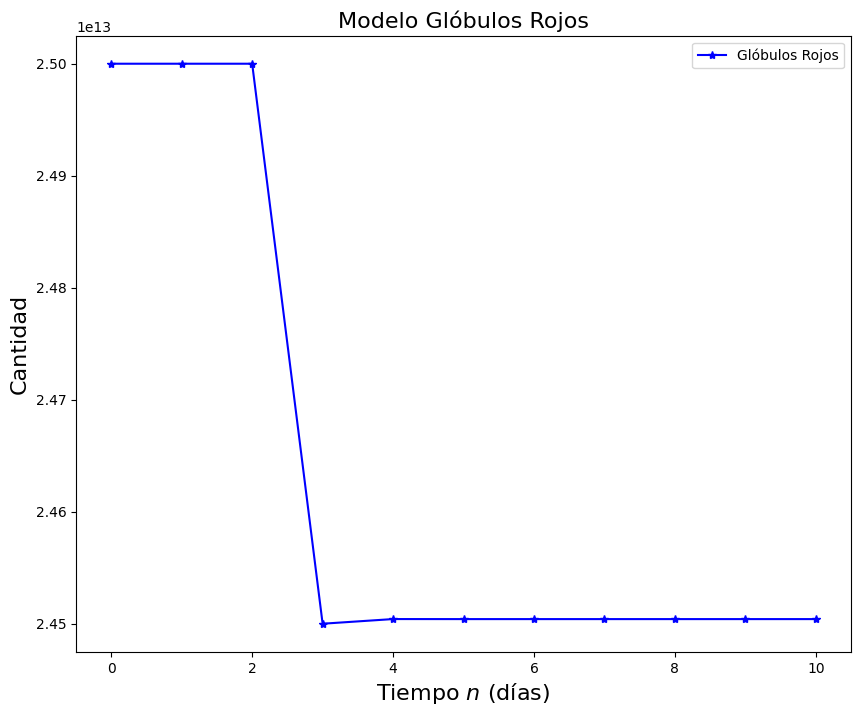
\includegraphics[scale=0.57]{figures/HemoLeveG1RBC.png}
    \caption{Caption?}
    \label{sec:variaciones:fig:HemoLeveG1RBC}
\end{figure}

\begin{figure}[H]
    \centering
    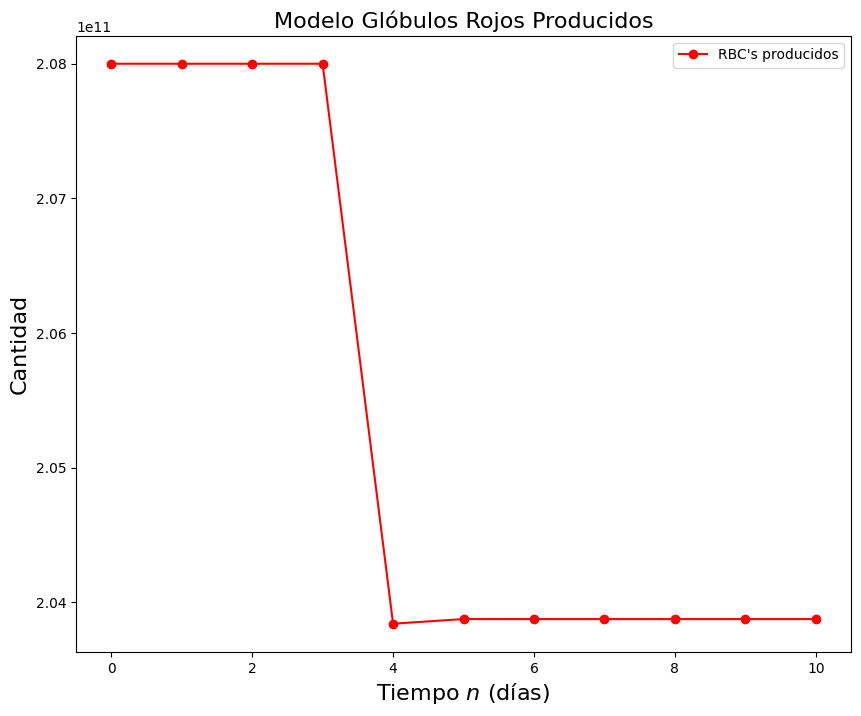
\includegraphics[scale=0.57]{figures/HemoLeveG1SC.png}
    \caption{Caption?}
    \label{sec:variaciones:fig:HemoLeveG1SC}
\end{figure}
